\documentclass[UTF8,a4paper]{ctexart}

% ==========Preamble==========
\usepackage{graphicx}
\usepackage{listings}
\usepackage{apacite}
\usepackage{url}
\usepackage{fancyhdr}
\usepackage{geometry}
\usepackage[font=small,labelfont=bf,labelsep=quad,format=hang,textfont=it]{caption}
\usepackage{booktabs}
\usepackage{graphicx}
\usepackage{float}
\usepackage{xcolor}
\usepackage{subfigure}
\usepackage{amsmath}
\DeclareMathOperator{\sign}{sign}

\definecolor{commentcolor}{RGB}{85,139,78}
\definecolor{stringcolor}{RGB}{206,145,108}
\definecolor{keywordcolor}{RGB}{34,34,250}
\definecolor{backcolor}{RGB}{220,220,220}

\pagestyle{plain}
\CTEXsetup[format=\Large\bfseries]{section}
\bibliographystyle{apacite}
\DeclareGraphicsExtensions{.eps,.pdf,.jpg,.png}

%设置代码
\lstset{
	%backgroundcolor=\color{red!50!green!50!blue!50},%代码块背景色为浅灰色
%	rulesepcolor= \color{gray}, %代码块边框颜色
    commentstyle=\color{commentcolor},	%注释颜色
	keywordstyle=\color{keywordcolor},	%关键词颜色
	stringstyle=\color{stringcolor},	%字符串颜色
	breaklines=true,  %代码过长则换行
	numbers=left, %行号在左侧显示
	numberstyle= \small,%行号字体
	%keywordstyle= \color{blue},%关键字颜色
	commentstyle=\color{gray}, %注释颜色
%	frame=shadowbox%用方框框住代码块
	frame=single,
	escapeinside=``    % 代码包含中文
}

% 设置图表搜索路径, 可以给图表文件夹取如下名字
\graphicspath{{img/}}

% ==========Title==========

\title{\bfseries 第四章作业 } 
\author{\bfseries 谈昊\quad2020E8013282037}

% Your name in the first blank and your additional information in \thanks{}
\date{}
% delete \today if you don't want the date

% ==========Document==========

\begin{document}
\maketitle


\paragraph{Answer}
\begin{itemize}
    \item[一、] 
    \begin{itemize}
        \item $$S_w=\left\{
            \begin{matrix}
                0.44444444 &-0.22222222 &-0.22222222 \\
                -0.22222222  &0.44444444 &-0.22222222 \\
                -0.22222222 &-0.22222222 & 0.44444444
            \end{matrix}\right\}
            $$
        \item $$S_b=\left\{
            \begin{matrix}
                0.7654321&  0.16049383  \\
                0.16049383& 0.7654321 
            \end{matrix}\right\}
            $$
    \end{itemize}
    
    
    \item[二、] 
    如下图:
        \begin{figure}[H]
            \centering
            \subfigure[2D]{
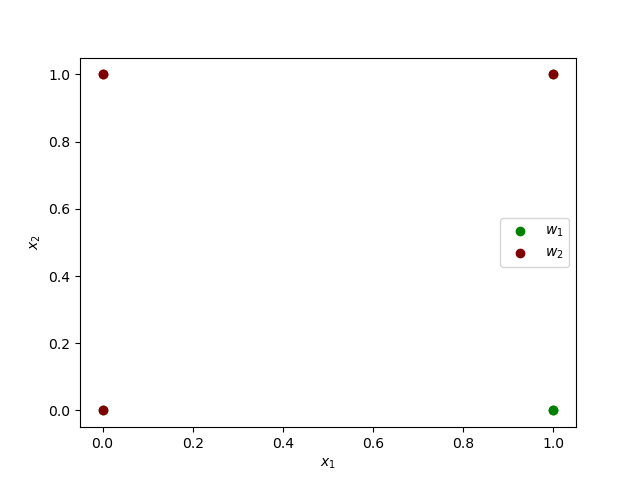
\includegraphics[width=0.45\textwidth]{KL_2D.png}
%\caption{fig1}
}
\subfigure[1D]{
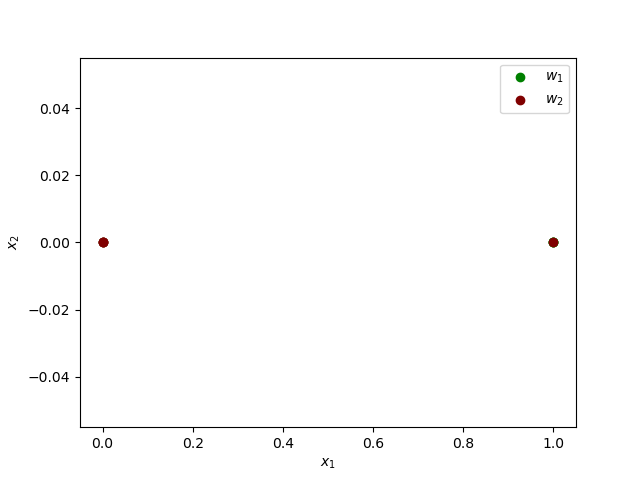
\includegraphics[width=0.45\textwidth]{KL_1D.png}
%\caption{fig1}
}
        \end{figure}
\end{itemize}

\end{document}

